\OriginalPage{129}{A Multiprocessor System Model}
\setcounter{chapter}{5}
\setcounter{section}{0}
\noindent{\LARGE\bfseries 5.\quad A Multiprocessor System Model\par}
\label{chap:multiprocessor-system}

\section{Introduction}
\label{sec:mp-introduction}

In earlier chapters, we discussed two smpl simulation models: a simple
single-server queueing system model and a two-class queueing network model.
In this chapter, we'll look at another example: a model of memory and bus
contention in a multiprocessor system. This example presents some new
modeling problems and further illustrates the use of smpl. We'll begin by
developing an analytic model of the system, and then develop a simulation
model to check the analytic results. After cross-verifying analytic and
simulation results, we'll consider ways of extending the simulation model to
eliminate some of the assumptions used in the analytic approach.

\section{The Multiprocessor System}
\label{sec:mp-system}

The system we'll be studying is diagrammed in Figure 5.1. It comprises $N$
processors and $M$ global memory modules (or, simply, memories)
interconnected by $B$ buses so that every processor can access every memory.
Transfers between processors and memories take place in fixed-size units
equal to the bus width, so that each transfer requires one bus cycle. The
system is synchronous: all memory requests are initiated at the same point in
a cycle.

We'll assume --- at least for now --- that the $N$ processors are physically
and functionally identical. Each processor has its own local memory, which
may be a cache or may take the form of data registers and an instruction
buffer. When executing, a processor issues an instruction fetch or an operand
fetch or store request in every machine cycle. This request is satisfied in the
processor's local memory with probability $h$ and requires access to (global)
memory with probability $p=1-h$. $h$ is called the hit ratio and $p$ is called
the miss ratio. Memory request processing takes place as follows.

\OriginalPage{130}{A Multiprocessor System Model}
\begin{figure}[H]
\centering
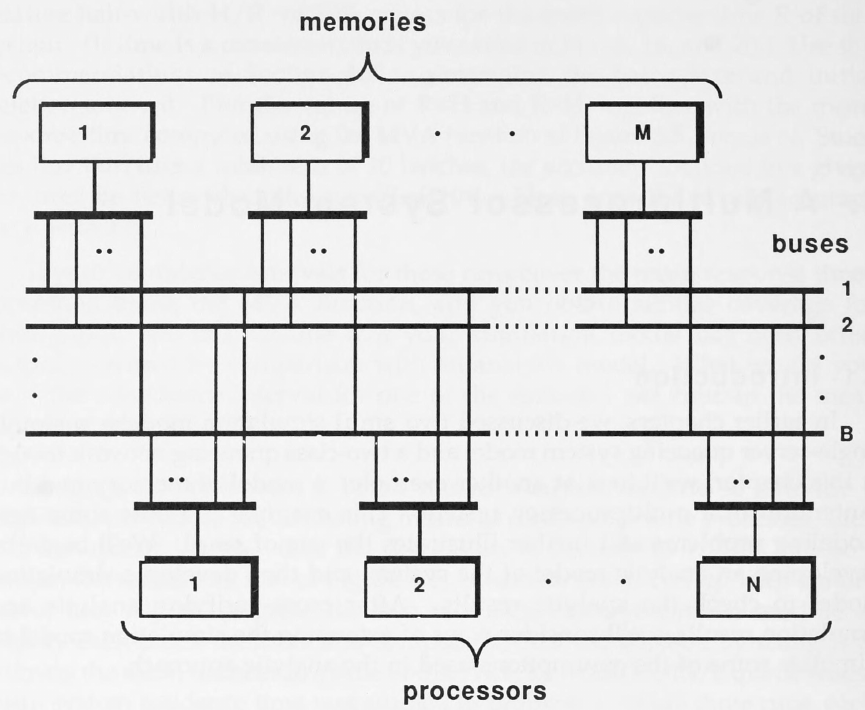
\includegraphics[width=.75\textwidth]{figures/ch5-system.png}
\caption{Multiprocessor System Elements}
\end{figure}

\begin{enumerate}
\item A processor initiates a memory request at the start of a machine cycle
and simultaneously suspends execution. Multiple requests for the same module
are resolved by an arbitration mechanism. We'll assume that this mechanism
tries to provide fair service via a cyclical scan of processors for requests,
with the scan starting point being advanced on each new scan.
\item If a request is successful, the module is reserved for the processor;
otherwise, the request is reissued at the start of the next cycle. From the
set of up to $M$ successful requests, a second arbitration mechanism selects
up to $B$ requests and reserves buses for these requests. We'll assume this is
done in the same order in which modules were reserved. If a request is
unsuccessful in obtaining a bus, the module is released and the request
reissued at the start of the next cycle.
\end{enumerate}
\OriginalPage{131}{5.3\quad An Approximate Analytic Model}
\begin{enumerate}
\setcounter{enumi}{2}
\item Next, for a successful request, the address and data, if the request is
a store, are transmitted over the bus to memory; if the request is a fetch,
data is returned over the bus at the end of the cycle.
\item When the bus cycle ends, processors whose requests were successfully
completed are returned to execution, and the buses and modules reserved by
these requests are released. Unsuccessful requests are reissued, together with
new requests, at the start of the next cycle.
\end{enumerate}

Our objective is to determine how processor performance is affected by
contention for memory modules and buses.

This system, in various forms, has received a great deal of attention over
the years. When the number of buses is equal to the number of memories
($B=M$), the interconnection between processors and memories is equivalent
to a crossbar network, and performance is affected only by memory contention.
Most of the early analysis work focused on this problem; most recent work
encompasses systems with $B<M$ and considers both bus and memory
contention.

\section{An Approximate Analytic Model}
\label{sec:mp-analytic-model}

The analytic model we'll develop in this section is based on that
described by Mudge et al. [1984]: the references in that paper provide a good
starting point for surveying work done in this area. There are several
measures of performance of interest to us; the one we'll look at first is the
system bandwidth, $BW$. This is the overall transfer rate between processors
and memory, expressed in terms of transfers per unit time. Since the transfer
time is 1 cycle, the overall bus utilization is (numerically but not
dimensionally) equal to $BW$, and $BW$ sometimes is defined as the average
number of busy buses.

The miss ratio $p$ was defined as the probability that a processor issues a
(global) memory request in a given cycle. If we assume that the probability
of issuing a request in any one cycle is the same as, and independent of, the
probability of issuing a request in any other cycle, then a processor's
execution interval corresponds to a sequence of Bernoulli trials. Execution
intervals therefore have a geometric distribution with mean $x=(1-p)/p$
and variance $\sigma^2=(1-p)/p^2$ (see, for example, Allen [1978] or Trivedi
[1982]). The geometric distribution is the discrete counterpart of the negative
exponential distribution. We'll also assume that memory requests are independ-
\OriginalPage{132}{A Multiprocessor System Model}
\noindent ently and uniformly distributed across memories (since memory module
selection typically is based on the low-order address bits).

Consider the long-term behavior of the system, looking first at those
cycles which have no reissued requests from the preceding cycle. Based on
the assumptions of the preceding paragraph, the probability that processor $i$
requests memory $j$ is $p/M$ for all $i$ and $j$. The probability that processor $i$ does
not request memory $j$ is $1-p/M$, and the probability that none of the $N$
processors requests memory $j$ is $(1-p/M)^N$. Therefore, the probability $q$ that
there is at least one request for memory $j$ is
\begin{equation}
q=1-(1-p/M)^N
\label{eq:mp-q-p}
\end{equation}

Assuming memory request probabilities are identical and independent, the
probability $f_i$ that exactly $i$ of $M$ memories have requests is binomial:\footnote{This is an approximation: note, for example, that $f_0$ should be 0 for $p=1$, while (5.1) and (5.2) give $f_0>0$. However, the error is small, even for $M$ as small as 4.}
\begin{equation}
f_i=\binom{M}{i}q^i(1-q)^{M-i}
\label{eq:mp-fi}
\end{equation}

The expected number of distinct memories requested in the cycle is $qM$.

While $qM$ requests may be presented to the bus arbitration mechanism in
a cycle, no more than $B$ requests can be granted. The expected number of bus
requests granted in a cycle --- equal numerically to the bandwidth --- is
\begin{equation}
BW=B\sum_{i=B}^{M} f_i+\sum_{i=1}^{B-1} i f_i
\label{eq:mp-bw}
\end{equation}

The bandwidth estimated from (5.1)--(5.3) applies only to cycles in which no
requests are reissued; in this case, the average request rate per processor is
the same as the miss rate $p$, and the overall request rate is $Np$. In the
general case, considering all cycles, the per processor request rate $r$ is greater
than the miss rate (since it comprises both initial and reissued requests). An
exact analysis is difficult; however, if we can estimate $r$, we can use it in
place of $p$ in (5.1) and obtain an improved estimate of $BW$.

Now look at the processor inter-request interval --- the interval between
two successful memory request completions --- shown in Figure 5.2. The mean
overall length of this interval is $T$. We can divide $T$ into three parts: an
execution interval of mean length $x=(1-p)/p$, a delay interval whose mean
\OriginalPage{133}{5.3\quad An Approximate Analytic Model}
\begin{figure}[H]
\centering
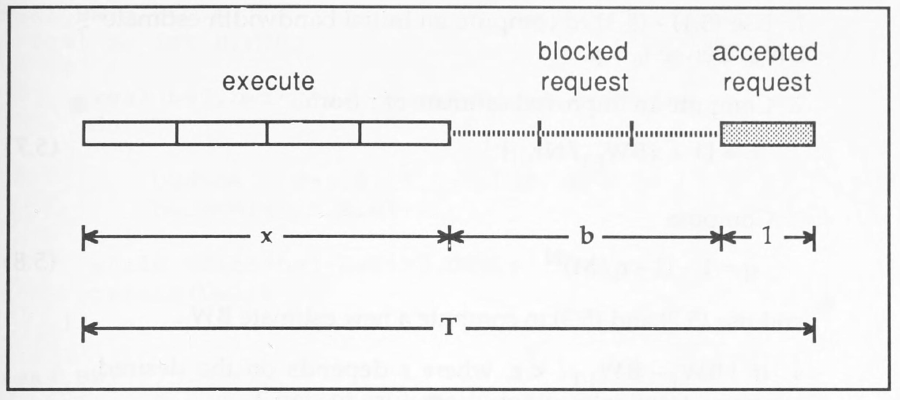
\includegraphics[width=.9\textwidth]{figures/ch5-interval.png}
\caption{Processor Inter-Request Interval Timing}
\end{figure}
\noindent length is defined as $b$, and a 1-cycle transfer time for the accepted request. $b$
represents the delay incurred when a request is blocked and reissued in the
succeeding cycle. The single processor request rate (counting both blocked and
accepted requests) is



\begin{equation}
r=(b+1)/T=(b+1)/(x+b+1)
\end{equation}
dividing numerator and denominator by $b+1$,
\begin{equation}
r=[1+x/(b+1)]^{-1}
\end{equation}
Since $r$ represents both blocked and accepted requests, $b+1=rT$ is the total
number of requests issued in $T$. The per processor request completion rate is
$BW/N$: the reciprocal of this rate is the mean interval between completed
requests $T$, so $T=N/BW$ and $b+1=Nr/BW$. Substituting the last for $b+1$
in (5.5),
\begin{equation}
r=[1+xBW/Nr]^{-1}
\end{equation}
(5.6) defines $r$ as a function of $r$ (both directly and indirectly, since $BW$ is a
function of $r$), and can be used in a simple fixed-point iterative algorithm
(see, for example, Rice [1983]) to estimate $BW$. This algorithm works as
follows.

\OriginalPage{134}{A Multiprocessor System Model}
\begin{enumerate}
\item Use (5.1)--(5.3) to compute an initial bandwidth estimate
$BW_0$. Define $r_0=p$.
\item Compute an improved estimate of $r$ from
\begin{equation}
r_i=[1+xBW_{i-1}/Nr_{i-1}]^{-1}
\end{equation}
\item Compute
\begin{equation}
q=1-(1-r_i/M)^N
\end{equation}
and use (5.2) and (5.3) to compute a new estimate $BW_i$.
\item If $|BW_i-BW_{i-1}|<\epsilon$, where $\epsilon$ depends on the desired
accuracy, terminate; otherwise, return to step 2.
\end{enumerate}

A C implementation of this algorithm, with $\epsilon=0.005$, is given in Figure 5.3.
You'll need to provide a main program to call \texttt{BW()} with values of $p$, $B$, $M$, $N$,
and to report results. Timing diagram relationships, together with the
operational laws discussed in Section 1.4, can be used to obtain other
measures: let's look at some of these.



\noindent\textbf{Utilizations and waiting time.} The average utilizations of a single bus,
single memory module, and single processor are, respectively, $U_B=BW/B$,
$U_M=BW/M$, and $U_P=xBW/N$ (from the Utilization Law). The average
waiting (blocked) time per request is $b$: from Figure 5.2, $b=T-x-1$. Since
$T=N/BW$ and $x+1=1/p$,
\begin{equation}
b=(N/BW)-(1/p)
\end{equation}
We could also obtain this result via the Response Time Law (Section 1.4).
This law typically is presented in the context of a time-sharing system,
where it has the form
\begin{equation}
R=(N/X)-Z
\end{equation}
Here, $R$ is the mean response time at a terminal, $N$ is the number of
terminals, $X$ is the computer system throughput, and $Z$ is the mean think
time at a terminal (mean time between successive system requests). The
correspondence between this system and our multiprocessor system is
\begin{center}
\begin{tabular}{rcl}
computer system & --- & memory/bus subsystem \\
$N$ terminals & --- & $N$ processors \\
mean think time $Z$ & --- & mean execution interval $x$ \\
system throughput $X$ & --- & bandwidth $BW$ \\
mean response time $R$ & --- & mean request processing time $b+1$
\end{tabular}
\end{center}
\OriginalPage{135}{5.3\quad An Approximate Analytic Model}
\begin{figure}[H]
\centering
\begin{minipage}{.92\textwidth}
\begin{lstlisting}[basicstyle=\ttfamily\scriptsize]
real BW(p,B,M,N)
  real p; int B,M,N;
    {
      real bw0,bw1=p*N,r=p,x=1.0/p-1.0,BWi();
      do
        {
          bw0=bw1; r=1.0/(1.0+x*bw0/(N*r));
          bw1=BWi(r,B,M,N);
        }
      while (fabs(bw1-bw0)>0.005);
      return(bw1);
    }

real BWi(r,B,M,N)
  real r; int B,M,N;
    { /* compute bandwidth for request rate r */
      int i; real q,bw=0.0,f();
      q=1.0-pow(1.0-r/M,(real)N);
      for (i=1; i<B; i++) bw+=i*f(i,M,q);
      for (i=B; i<=M; i++) bw+=B*f(i,M,q);
      return(bw);
    }

real Fact(n)
  int n;
    { /* compute n factorial */
      real z=1.0;
      while (n) {z*=n; n--;}
      return(z);
    }

real C(n,k)
  int n,k;
    { /* compute binomial coefficient */
      return(Fact(n)/(Fact(k)*Fact(n-k)));
    }

real f(i,M,q)
  int i,M; real q;
    { /* compute binomial probability */
      real z;
      z=C(M,i)*pow(q,(real)i)*pow(1.0-q,(real)(M-i));
      return(z);
    }
\end{lstlisting}
\end{minipage}
\caption{Bandwidth Computation Algorithm}
\end{figure}
\OriginalPage{136}{A Multiprocessor System Model}
\noindent Making the appropriate substitutions in (5.10) results in (5.9).

\noindent\textbf{Mean queue length.} Let $L_b$ be the average number of blocked requests
outstanding per processor. From Little's Law,
\begin{equation}
L_b=bBW/N
\end{equation}
from which
\begin{equation}
L_b=1-BW/Np
\end{equation}
(5.12) also can be obtained as follows. In any given period of time, a processor
spends, on the average, proportions $U_P$ executing, $L_b$ waiting, and $BW/N$
transferring: thus, $U_P+BW/N+L_b=1$. Substituting for $U_P$ and subsequently
for $x$, and rearranging terms gives (5.12).

\noindent\textbf{System throughput.} While the bandwidth provides a direct measure of
memory-bus subsystem performance, it is only an indirect measure of system
performance. For a given configuration ($B$, $M$, $N$), a processor design change
which increases the miss rate will result in an increase in $BW$ but reduced
system throughput. Suppose the unit of work in this system is a task, and
each task requires an average of $n$ execution intervals: the average service
time per task, then, is $nx$. From the Utilization Law, the system throughput
is $N[U_P/nx]$ tasks per unit time. For design comparisons, it may be useful to
work with the \emph{normalized} system throughput $\eta$, obtained by taking $nx=1$:
\begin{equation}
\eta=NU_P=N[xBW/N]=BW[(1/p)-1]
\end{equation}
Note that if there are no contention delays, $BW=Np$ and $\eta=N(1-p)$, and
if the miss rate $p$ is zero, $\eta=N$.

Our bandwidth analysis is approximate because, among other things, it
assumes that memory request probabilities are independent in (5.1) and (5.2).
This is equivalent to assuming that a request blocked on access to module $j$ is
assigned at random to one of the $M$ modules when reissued. In the actual
system, a blocked request for module $j$ is reissued to module $j$, so the probability
that module $j$ is referenced in cycle $n$ is not independent of whether or
not it was referenced in cycle $n-1$. In the next section, we'll look at a
simulation model which can be used to verify the approximate analytic
model and also evaluate the effect of this independence assumption.

\section{Verifying the Analytic Model}
\label{sec:mp-verify}

The kind of simulation model we develop for analytic model verification
depends on our objectives. In the case of the multiprocessor system, our
\OriginalPage{137}{5.4\quad Verifying the Analytic Model}
\noindent objective is to verify that the analytic model adequately represents the
behavior of the system, so the simulation model reflects the structure of the
system. Sometimes, though, our objective may be to check the assumptions
and mathematics of the analysis itself, and our model may be much more
abstract in form. As a simple example of this case, suppose we need to determine
the average seek distance on a disk. We assume disk requests are
independently and uniformly distributed across the $C$ cylinders of a disk,\footnote{This assumption frequently has been shown to be invalid in practice: see, for example, McNutt [1984].}
and our derivation results in an average seek distance of approximately $C/3$.
We can verify this result via a simple simulation in which we generate a
sequence of random numbers $X_1, X_2, \ldots$, each of which is uniformly distributed
in $[1,C]$, and compute the average absolute difference $|X_i-X_{i-1}|$. This type
of checking is a great help in catching mistakes in analytic models; we may
not be able to apply it to a model as a whole, but often can use it to check
individual steps.

A smpl simulation model developed to validate our analytic model is
shown in Figure 5.4; for reference purposes, we'll call this model \emph{bws1}. This
model defines memory modules and buses as smpl facilities, while processors
are represented as tokens. Global declarations define the miss rate $p$, the
number of processors $N$, the number of memory modules $M$, and the number of
buses \texttt{nB} (remember that \texttt{B} is a smpl function name), together with the
facility descriptors \texttt{module[]} and \texttt{bus}. \texttt{treq[n]} is used to record the next
memory request issue time for processor $n$, and \texttt{req[n]} to record the module
number of a request; \texttt{tn}, the earliest-occurring request time, is initialized to
a large value.

Model initialization is straightforward. \texttt{smpl()} is called to initialize
the simulation subsystem, facilities are declared, \texttt{next\_access()} is called
to determine the initial access time for each processor and to compute \texttt{tn}, and
the first event is scheduled at time \texttt{tn}. Each memory module is defined as a
single-server facility, while the set of buses is defined as a multiserver
facility; since any bus can be used for a transfer, buses need not be distinguishable.

The \texttt{next\_access()} function generates a processor execution interval by
generating a random variate from a geometric distribution with mean
$(1-p)/p$; it then adds this interval to the current simulation time to obtain
the simulation time at which the processor's next memory request is to be
issued. (Note that \texttt{treq[n]} is an event occurrence time, not an inter-event
time.) If the request issue time \texttt{t} computed for processor $n$ is less than the
\OriginalPage{138}{A Multiprocessor System Model}
\begin{figure}[H]
\centering
\begin{minipage}{.98\textwidth}
\begin{lstlisting}[basicstyle=\ttfamily\scriptsize]
#include <smpl.h>
#define busy 1

real
  p=0.250,         /* local memory miss rate                */
  treq[17],        /* next request time for processor       */
  tn=1.0E6;        /* earliest-occurring request time       */
int
  N=8,M=4,nB=2,    /* no. processors, memories, & buses     */
  module[17],bus,  /* memory & bus facility descriptors     */
  nbs=0,           /* no. busy buses in current cycle       */
  req[17],         /* currently-requested memory module     */
  next=1;          /* arbitration scan starting point       */

/*------------  MEMORY-BUS BANDWIDTH MODEL  ------------*/
main()
  {
    int event,i,n;
    smpl(0,"Bandwidth Model");
    bus=facility("bus",nB);
    for (i=1; i<=M; i++) module[i]=facility("module",1);
    for (n=1; n<=N; n++) {req[n]=0; next_access(n);}
    schedule(1,tn,0);
    while (time()<10000.0)
      {
        cause(&event,&n);
        switch(event)
          {
            case 1: begin_cycle(); break;
            case 2: req_module(n); break;
            case 3: end_cycle(n);  break;
          }
      }
    printf("BW = %.3f\n",U(bus));
  }

/*-------------  COMPUTE NEXT ACCESS TIME  -------------*/
next_access(n)
  int n;
    {
      real t;
      t=floor(log(ranf())/log(1.0-p))+time();
      treq[n]=t; if (t<tn) then tn=t;
    }
\end{lstlisting}
\end{minipage}
\caption{Multiprocessor Simulation Model \emph{bws1}}
\end{figure}
\OriginalPage{139}{5.4\quad Verifying the Analytic Model}
\addtocounter{figure}{-1}
% PDF page 161 (printed 139): the listing prints no closing parenthesis
% after module[req[n]] in the status test, and a colon after req[n]=0.
% Both apparent source typographical errors are retained verbatim.
\begin{figure}[H]
\centering
\begin{minipage}{.98\textwidth}
\begin{lstlisting}[basicstyle=\ttfamily\scriptsize]
/*--------------  EVENT 1: BEGIN CYCLE  ---------------*/
begin_cycle()
  {
    int i,n=next; real t,tmin=1.0E6;
    for (i=0; i<N; i++)
      {
        if (!req[n]) then
          { /* in this version, req[n] always is 0 here */
            if ((t=treq[n])==tn)
              then
                {req[n]=random(1,M); schedule(2,0.0,n);}
              else if (t<tmin) then tmin=t;
          }
        n=(n%N)+1;
      }
    next=(next%N)+1; tn=tmin;
  }

/*---------  EVENT 2: REQUEST MEMORY AND BUS  ---------*/
req_module(n)
  int n;
    {
      if (status(module[req[n]]!=busy&&status(bus)!=busy)
        then
          {
            request(module[req[n]],n,0); request(bus,n,0);
            nbs++; schedule(3,1.0,n);
          }
        else
          {req[n]=0; if (++treq[n]<tn) then tn=treq[n];}
    }

/*---------------  EVENT 3: END CYCLE  ----------------*/
end_cycle(n)
  int n;
    {
      release(bus,n); release(module[req[n]],n);
      req[n]=0: next_access(n);
      if (--nbs==0) then schedule(1,tn-time(),0);
    }
\end{lstlisting}
\end{minipage}
\caption{Multiprocessor Simulation Model \emph{bws1} (continued)}
\end{figure}
\OriginalPage{140}{A Multiprocessor System Model}
\noindent current earliest-occurring request time \texttt{tn}, \texttt{tn} is set to \texttt{t}. A geometric variate
is generated by the expression
\begin{center}
\texttt{floor(log(ranf())/log(1-p))}
\end{center}
This is obtained from the inverse distribution function of the geometric
distribution (see problem 2(c), Chapter 1). Because of the use of the \texttt{floor()}
function, simulation times will be non-fractional.





The major difference between this model and the simulation models of
Chapters 1 and 2 is its synchronous operation. In this model, the unit of time
is the bus cycle; time advances in integer multiples of this unit, and events
occur either at the beginning or at the end of a cycle. Since the end of one
cycle corresponds to the beginning of the next and so are the same instant in
simulation time, we can't rely on the event list to insure that events occur in
the proper order. In this model, order is maintained by ``batching'' memory
request initiations and completions. There are a variety of other ways to
accomplish this. For example, in the actual system, a bus cycle divides into
some number of clock cycles. Using the clock cycle as the unit of time would
solve the problem, since the beginning of bus cycle $n$ would occur at a later
clock cycle than the end of bus cycle $n-1$. Another possibility is to extend the
event list mechanism to provide $T-$ and $T+$ scheduling (i.e., to recognize the
beginning and end of a time unit).

The model proper comprises three event routines:\newline
\texttt{begin\_cycle()},
\texttt{req\_module()}, and \texttt{end\_cycle()}. At any point during the simulation,
\texttt{treq[n]} is the next request issue time for processor $n$, and \texttt{tn} is the earliest-
occurring request issue time. Event 1 is scheduled to occur at time \texttt{tn} as part of
model initialization and, subsequently, by \texttt{end\_cycle()}. \texttt{begin\_cycle()}
scans the set of $N$ processors for those issuing requests at time \texttt{tn} and, for each
such processor, assigns a random memory module as the request destination
and schedules the memory (and bus) request, event 2. This check is made only
for processors for which \texttt{req[n]} is zero: this always is true for model \emph{bws1}
(but not for the variant we'll look at in the next section). Each scan of the
processor set begins with processor \texttt{next}, which is advanced at the end of
each scan. This represents the arbitration mechanism of the system more
closely than it does the assumed random processor selection of our analytic
model. However, it is more efficient to simulate than random processing,
introduces less bias than a $1$--$N$ scan, and has little effect on the results. As
\texttt{begin\_cycle()} does its scan, it keeps track of the earliest-occurring request
issue time following \texttt{tn} and, at the end of the scan, updates \texttt{tn} to this time.

\texttt{begin\_cycle()} schedules event 2 for each processor it finds with a
request issue time of \texttt{tn}: this event, like event 1, occurs at the beginning of a
cycle. The event 2 routine, \texttt{req\_module()}, checks to see if the requested
\OriginalPage{141}{5.4\quad Verifying the Analytic Model}
\noindent memory module is free and if a bus is free. If these conditions are met, the
module and a bus are reserved, the number of buses busy in this cycle, \texttt{nbs}, is
incremented, and completion of the request is scheduled to occur at the end of
the cycle. (Note that the inter-event time is 1.) If the requested module is
busy or if a bus cannot be obtained, the request is blocked for reissue at the
start of the next cycle: \texttt{req[n]} is set to zero and the request issue time
\texttt{treq[n]} is incremented. If this new request issue time is less than \texttt{tn}, \texttt{tn} is
adjusted accordingly. When the request is reissued, a memory module will
selected at random for it, thus satisfying the independence assumption of our
analytic model.

Event 3 marks the completion of a request at the end of a bus cycle. The
bus and memory module are released, \texttt{req[n]} is set to zero, and
\texttt{next\_access()} is called to compute the next request issue time for the processor.
\texttt{nbs} is decremented and, if end-of-cycle processing is complete for all
bus transfers initiated in the current cycle (\texttt{nbs} = 0), event 1 is scheduled at
time \texttt{tn}. The \texttt{nbs} count provides the basic mechanism for the request
``batching'' mentioned earlier. Note that, since \texttt{tn} is an event occurrence
time, the current simulation time has to be subtracted from it in making the
\texttt{schedule()} call.

At the end of the simulation interval specified in the \texttt{while} statement
in \texttt{main()}, the utilization of the bus is printed as the bandwidth and model
execution then is terminated. Remember that bus utilization and bandwidth
are numerically the same only because the bus service time is 1.

The simulation model in Figure 5.4 was coded for compactness and can be
improved in several ways. Its performance can be improved by the use of
pointers, and by precomputing the factor \texttt{1.0/(1.0-p)} in geometric variate
generation. Its usefulness can be improved by providing a procedure to read
values of the input parameters \texttt{nB}, $M$, $N$, and $p$ (with SMPL, they can be
defined as SMPL parameters and their values then specified via the parameter
display). Finally, procedures for specifying the desired accuracy and
determining the requisite run length are needed.

\noindent\textbf{Output analysis.} Methods of determining the run length required to
achieve a specified simulation accuracy were discussed in Chapter 4. A
sequential procedure using the batch means method was recommended, and a
set of procedures implementing this method for a discrete-time output
variable was presented in Figure 4.7. In our present problem, the simulation
output variable --- the bandwidth --- is a continuous-time variable, so the
procedures of Figure 4.7 can't be used directly. However, a similar approach
can be used, and the code will be even simpler, since collection of values for
and computation of individual batch means doesn't have to be done. For a
continuous-time variable, the batch size is defined as a fixed-length simu-
\OriginalPage{142}{A Multiprocessor System Model}
\noindent lation interval $t$. The model schedules an event every $t$ cycles and, when the
event occurs, calls \texttt{U(bus)} to get the bandwidth --- the current batch mean ---
for the interval, and then calls \texttt{reset()} to reinitialize smpl's counters and
accumulators. Given that at least two batch means have been collected, a
confidence interval can be computed and the relative half-width compared
with the required accuracy to determine whether to terminate the run or to
go on and collect another batch. You'll find extending the batch means
analysis module of Figure 4.7 to handle continuous-time as well as discrete-
time output variables is not only a good exercise but also a worthwhile
enhancement to your set of simulation tools. (See problem 4, Chapter 4.)

When using simulation to verify analytic results, we'll frequently want
to use tighter confidence intervals and higher confidence levels than we
would in problem analysis so that differences in results due to inherent
differences in the two models won't be attributed to sampling variation.
(This desire is tempered by the run lengths which may result.) The author's
simulations of this system were performed using the sequential batch means
procedure discussed above with a specified confidence level and relative
half-width of, respectively, 99 percent and 1 percent, a batch ``size'' of 1000
cycles, and a minimum number of batches equal to 10. Over the range of
parameters studied ($2\le N\le16$, $N/2\le M\le N$, $1\le B\le M$, $0.1\le p\le1$), the desired
accuracy was obtained with the minimum number of batches. Long runs were
not required because the coefficient of variation of bus utilization is low: the
system is closed, the population (in the study range) is low, and the service
time is constant.

\noindent\textbf{Comparison of results.} Our multiprocessor model has four parameters:
three are discrete-valued and one ($p$) is continuous-valued. If we limit
verification to the parameters mentioned in the preceding paragraph, using
an increment of 0.1 for $p$, checking each parameter value combination will
require an extremely large number of runs: 30 runs would be required just for
$N=2$. (How many would be required at $N=16$?) An exhaustive comparison
of analytic and simulation results, then, probably is not feasible; we need to
find a more selective approach.\footnote{While in this case we want to verify an analytic model (the test model) against a simulation model (the base model), the same problem arises when their roles are reversed so that the simulation model is the test model and the analytic model is the base model.}

One thing we can do is plot the analytic results to see how $BW$ changes
with changes in parameter values, and concentrate our verification efforts on
the more ``interesting'' points. What are these? Consider Figure 5.5, which
\OriginalPage{143}{5.4\quad Verifying the Analytic Model}
\begin{figure}[H]
\centering
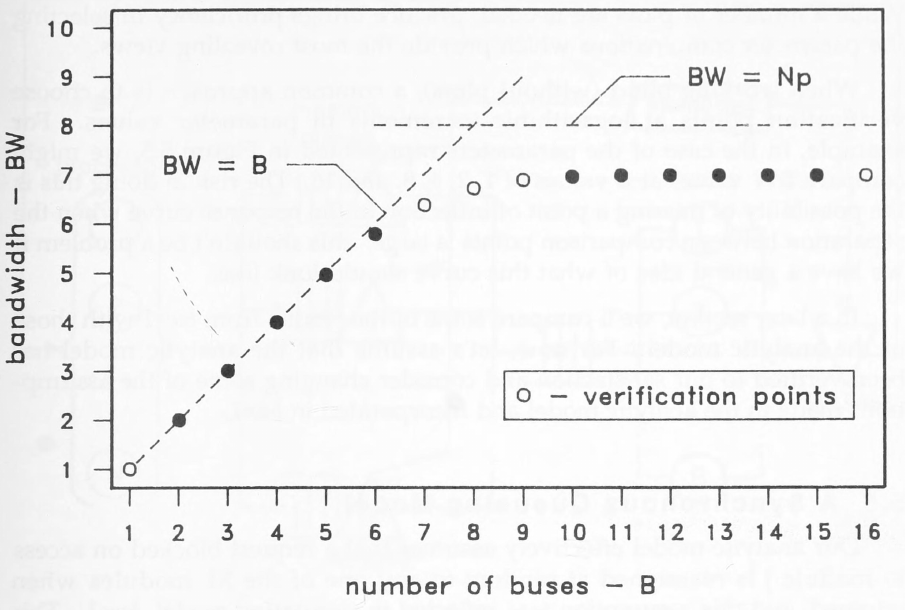
\includegraphics[width=.9\textwidth]{figures/ch5-bandwidth.png}
\caption{Bandwidth Versus No. of Buses for $N=M=8$, $p=0.5$}
\end{figure}
\noindent plots bandwidth versus the number of buses, $B$, for $M=N=8$ and $p=0.5$. When
the number of buses is small, the bandwidth is bus-limited (the buses are
said to be saturated), and $BW=B$. The test model probably will yield this
result for small values of $B$ even if it's not a very good model. In the case at
hand, we can verify this by inspection: we don't need to run a simulation. As
the number of buses becomes large, bus delays become small and $BW$
approaches a limit determined by memory delays: this limit is parallel to
the contention-free bandwidth $Np$. Since the rate of change in this range is
very small, we can limit our comparison to the endpoint $B=16$. The
interesting points are those for $B=7,8$ and $9$: the points which fall between
the region in which $BW$ is bus-limited and the region in which it is memory-
limited. If the test and base model results at these points and at endpoints
are in close agreement, further verification effort probably should be
directed elsewhere in the parameter space.



In this approach, each plot usually is generated as a set of curves (e.g.,
$BW$ versus $B$ for $p=0.1,0.2,\ldots,1.0$), and so gives us a kind of two-dimensional
view of what, in this case, is a four-dimensional response surface. (If you
have actual three-dimensional plotting capability, so much the better!)

\OriginalPage{144}{A Multiprocessor System Model}
\noindent While a number of plots are needed, practice brings proficiency in selecting
the parameter combinations which provide the most revealing views.

When working blind (without plots), a common approach is to choose
verification points at logarithmic increments in parameter values. For
example, in the case of the parameters represented in Figure 5.5, we might
compare $BW$ values at $B$ values of 1, 2, 4, 8, and 16. The risk in doing this is
the possibility of missing a point of inflection in the response curve when the
separation between comparison points is large; this shouldn't be a problem if
we have a general idea of what this curve should look like.

In a later section, we'll compare some of the results from \emph{bws1} with those
of the analytic model. For now, let's assume that the analytic model has
been verified to our satisfaction and consider changing some of the assumptions
made in the analytic model and incorporated in \emph{bws1}.

\section{A Synchronous Queueing Model}

Our analytic model effectively assumes that a request blocked on access
to module $j$ is reassigned at random to any one of the $M$ modules when
reissued, and this assumption was reflected in simulation model \emph{bws1}. This
assumption easily is removed from \emph{bws1}: delete the statement \texttt{req[n]=0} in
\texttt{req\_module()} and, in \texttt{begin\_cycle()}, delete the \texttt{if (!req[n])} statement
and add an \texttt{if} statement to select a module for the processor's request
only if \texttt{req[n]} is zero. The resulting model provides more or less random
selection of requests for queues and buses, while the actual system may
provide some type of request queueing. To see how much effect this has on
performance, let's look at a model of the system in which module and bus
requests are queued on a first-in, first-out basis.

\noindent\textbf{Model diagram.} A queueing model for the system is diagrammed in
Figure 5.6. While this is a closed queueing network like that of Figure 2.1,
the symbols are new. In Figure 2.1, each symbol represents a simple single-
server queue at which requests arrive, queue for service, reserve the server,
receive service, release the server, and depart. In Figure 5.6, processors are
represented by a \emph{delay server}, whose symbol is a set of circles enclosed in
braces. (This sometimes is called an \emph{infinite server}.) A delay server always
has enough servers to accommodate requests and so has no queueing: requests
arrive, receive service, and depart. The terminals of a timesharing system
model can be viewed as a delay server, with the service corresponding to
think times. In the multiprocessor system model, this service corresponds to
processor execution intervals. Generally, we won't use a smpl facility to
represent a delay server unless we need to directly determine its utilization;
in this case, we can represent it by a facility set whose size is sufficient to
\OriginalPage{145}{5.5\quad A Synchronous Queueing Model}
\begin{figure}[H]
\centering
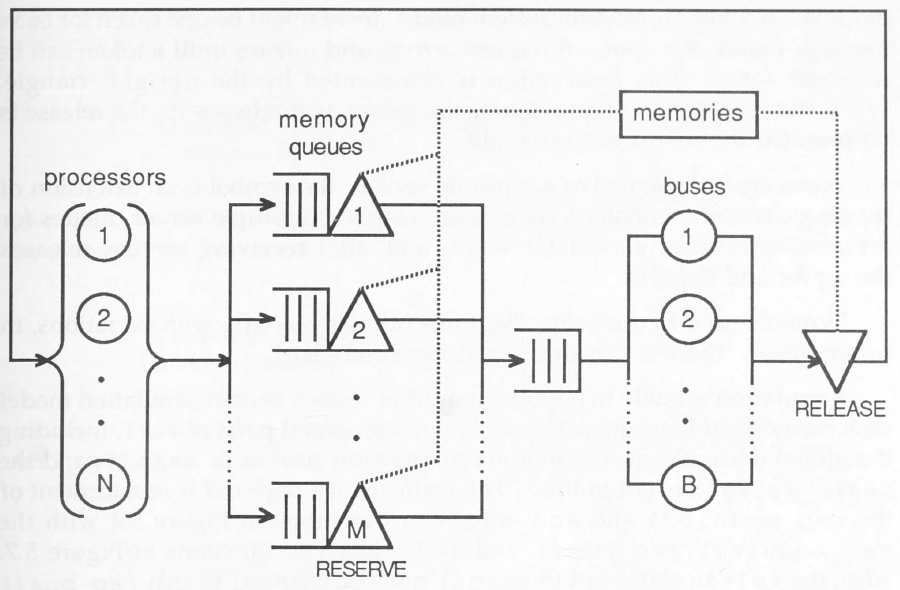
\includegraphics[width=.9\textwidth]{figures/ch5-queue-model.png}
\caption{Multiprocessor System Queueing Model Diagram}
\end{figure}
\noindent prevent queueing. (This, however, increases simulation overhead. It usually
is more efficient to measure the throughput and mean service time, and
compute the utilization via the Utilization Law.)



When a processor issues a memory request, the request queues for the
selected memory module, reserves it, queues for the bus, and reserves the bus.
The bus transfer is performed, the bus is released, and the memory module
then released. The memory module and the bus must be simultaneously
reserved to perform the transfer. This \emph{simultaneous resource possession} frequently
occurs in computer systems (and complicates the analytic solution of
queueing network models of these systems: for a discussion in the context of a
memory-bus contention model, see Jacobson and Lazowska [1981]). Other
examples of simultaneous resource possession include the simultaneous
reservation of a disk, control unit, and channel required for data transfer in
an IO operation, and the simultaneous reservation of memory space and
processor in executing a task. The symbols representing memory operations in
Figure 5.6 indicate that queueing and reservation operations are disjoint from
release. The interpretation of the symbols is as follows. Upon creation, the
box (labeled ``memories'' here) has $m$ tokens, each corresponding to an
allocatable resource unit. In this model, there is one token for each memory
\OriginalPage{146}{A Multiprocessor System Model}
\noindent module; in a communication system model, there might be one token for each
message buffer at a node. A request arrives and queues until a token can be
reserved for it: this reservation is represented by the upright triangle.
When the request no longer requires the resource, it releases it: the release is
represented by the inverted triangle.

Buses are represented as a multiple server: the symbol is an extension of
the single server symbol. A request arriving at a multiple server queues for
services, reserves any available server and, after receiving service, releases
the server and departs.

Symbols used in queueing diagrams in this book are, with variations, in
common use. There is, however, no accepted standard.

\noindent\textbf{Simulation model.} In building a multiprocessor system simulation model
with memory and bus queueing, we can reuse several parts of \emph{bws1}, including
the global declarations, the model initialization section in \texttt{main()}, and the
\texttt{begin\_cycle()} event routine. The main change required is replacement of
the \texttt{req\_module()} and \texttt{end\_cycle()} functions in Figure 5.4 with the
\texttt{req\_module()}, \texttt{req\_bus()}, and \texttt{end\_cycle()} functions of Figure 5.7.
Also, the \texttt{switch} statement in \texttt{main()} must be changed so that \texttt{req\_bus()}
is called on event 3 and \texttt{end\_cycle()} is called on event 4. Finally,
replacing the \texttt{printf} statement in \texttt{main()} with a call to \texttt{report()} will
provide mean memory and bus queue lengths, in addition to utilizations.
We'll call the model resulting from these modifications \emph{bws2}.

\emph{bws2}, like \emph{bws1}, is a synchronous model. Time advances in units of a bus
cycle, memory requests are initiated at the beginning of a cycle, and transfers
complete at the end of a cycle. \texttt{begin\_cycle()} scans processors for requests
just as it did in \emph{bws1}; in \emph{bws2}, however, processors which have requests
queued for a memory module or a bus will have \texttt{req[n]} non-zero, and so will
be skipped in this scan. For each processor which has a request to be issued
at the current time, a memory module is selected and event 2 scheduled.

In \texttt{req\_module()}, the event routine for event 2, the request is queued if
its memory module is busy; otherwise, the module is reserved and event 3
scheduled. In the event routine for this event, \texttt{req\_bus()}, a bus is requested.
If no bus is available, the request is queued. If a bus is available, it is
reserved, the count \texttt{nbs} of the number of busy buses in this cycle is incremented,
and the transfer completion, event 4, is scheduled.

The event 4 routine, \texttt{end\_cycle()}, is called as each bus request issued in
the current cycle completes. It changes \texttt{req[n]} to a negative value to
indicate that processor $n$'s request is complete, and decrements \texttt{nbs}. When
\texttt{nbs} reaches 0 (all current bus requests complete), \texttt{end\_cycle()} scans the set
of processors for those with completed requests and, for each such processor,
\OriginalPage{147}{5.5\quad A Synchronous Queueing Model}
\begin{figure}[H]
\centering
\begin{minipage}{.95\textwidth}
\begin{lstlisting}[basicstyle=\ttfamily\footnotesize]
/*-------------  EVENT 2: REQUEST MEMORY  -------------*/
req_module(n)
  int n;
    {
      if (request(module[req[n]],n,0)==0) then
        schedule(3,0.0,n);
    }

/*--------------  EVENT 3: REQUEST BUS  ---------------*/
req_bus(n)
  int n;
    {
      if (request(bus,n)==0) then
        {nbs++; schedule(4,1.0,n);}
    }

/*---------------  EVENT 4: END CYCLE  ----------------*/
end_cycle(n)
  int n;
    {
      req[n]=-req[n]; nbs--;
      if (nbs==0) then
        {
          for (n=1; n<=N; n++)
            if (req[n]<0) then
              {
                release(bus,n);
                release(module[-req[n]],n);
                req[n]=0; next_access(n);
              }
          schedule(1,tn-time(),0);
        }
    }
\end{lstlisting}
\end{minipage}
\caption{Changes to \emph{bws1} for Memory and Bus Queueing}
\end{figure}
\noindent releases the bus and the memory module, sets \texttt{req[n]} to zero, and calls
\texttt{next\_access()} to compute the next request time for the processor. When
this scan is complete, event 1 is scheduled to issue the next batch of requests.



A key difference between \emph{bws1} and \emph{bws2} is that, in the latter, release
operations are deferred until all bus requests issued in the current cycle have
completed. If this was not done, then releasing a bus, for example, might
cause a queued request to be dequeued and rescheduled for event 3, where it
would increment \texttt{nbs} and make this count invalid. As implemented in
Figure 5.7, all requests issued in the current cycle are allowed to complete,
\OriginalPage{148}{A Multiprocessor System Model}
\noindent and release operations then performed. This --- conceptually --- marks the
end of the current cycle. The release operations may cause queued requests to
be dequeued and rescheduled which --- again, conceptually --- occurs at the
beginning of the next cycle, and \texttt{begin\_cycle()} may schedule additional
requests at this time.

Bandwidths from \emph{bws1} and \emph{bws2} agree closely over a wide range of
parameter values (although not the entire range): we'll look at some results
later. One advantage of \emph{bws2} is that the mean delay per request, $b$, can be
decomposed into memory delays and bus delays.

\section{An Asynchronous Queueing Model}

\emph{bws1} and \emph{bws2} were constructed to represent the synchronous operation of
a real system: both models used fixed-unit time advancement and carefully
aligned request initiation and completion on cycle endpoints. This construction
also seemed to be a natural counterpart of the analytic model developed
in Section 5.3, which focused on the probability distributions of the number of
memory and bus requests made in a cycle. However, queueing network models
have been used with some success to model multiprocessor systems, and these
have not been constrained to represent synchronous behavior.\footnote{See, for example, Jacobson and Lazowska [1981], Smilauer [1985], and Towsley [1986].} It is
interesting, then, to see how results from an asynchronous queueing model
compare with those of our synchronous models.

An asynchronous simulation model of a multiprocessor system is shown in
Figure 5.8: we'll call it \emph{bws3}. It is another possible realization of the
queueing model diagram of Figure 5.6. \emph{bws3} is derived from, and is a simplification
of, \emph{bws2}. The code involved with batching request initiation and
completion operations has been discarded: since this left only a handful of
statements, the event routines were integrated into \texttt{main()}. The distribution
used to generate processor execution intervals has been changed from
geometric to exponential, since we're not concerned about producing integer-
valued execution times. \texttt{x} represents the mean execution interval; note that
its value is computed when it is declared.







\section{Model Results}

We now have an analytic model and three simulation models of this
system: let's look at some of the model results.
\OriginalPage{149}{5.6\quad An Asynchronous Queueing Model}
% PDF page 171 (printed 149): the listing omits a closing parenthesis in
% schedule(1,expntl(x),n;}, prints a semicolon after switch(event), and
% omits the case 1 label. These apparent source errors are retained.
\begin{figure}[H]
\centering
\begin{minipage}{.98\textwidth}
\begin{lstlisting}[basicstyle=\ttfamily\scriptsize]
#include <smpl.h>
#define queued 1

real p=0.250;     /* local memory miss rate                */
int  N=8,M=4,nB=2,/* no. processors, memories, & buses     */
     module[17],  /* facility descriptors for modules      */
     bus,         /* facility descriptor for buses         */
     req[17];     /* currently-requested memory module     */

/*------------  MEMORY-BUS BANDWIDTH MODEL  ------------*/
main()
  {
    int event,i,n; real x=1.0/p-1.0;
    smpl(0,"Bandwidth Model");
    bus=facility("bus",nB);
    for (i=1; i<=M; i++) module[i]=facility("module",1);
    for (n=1; n<=N; n++)
      {req[n]=random(1,M); schedule(1,expntl(x),n;}
    while (time()<10000.0)
      {
        cause(&event,&n);
        switch(event);
          {
              if (request(module[req[n]],n,0)!=queued)
                then schedule(2,0.0,n);
            break;
          case 2: /* reserve bus & initiate transfer  */
            if (request(bus,n,0)!=queued) then
              schedule(3,1.0,n);
            break;
          case 3: /* complete: schedule next request */
            release(bus,n);
            release(module[req[n]],n);
            req[n]=random(1,M);
            schedule(1,expntl(x),n);
          break;
          }
      }
    report();
  }
\end{lstlisting}
\end{minipage}
\caption{Multiprocessor Simulation Model \emph{bws3}}
\end{figure}
\OriginalPage{150}{A Multiprocessor System Model}
\begin{table}[H]
\centering
\begin{tabular}{rrrrrrrr}
\multicolumn{4}{c}{parameters} & \multicolumn{4}{c}{bandwidth} \\
$N$ & $M$ & $B$ & $p$ & \emph{bwa} & \emph{bws1} & \emph{bws2} & \emph{bws3} \\
4 & 4 & 4 & 1.000 & 2.734 & 2.739 & 2.619 & 2.613 \\
4 & 4 & 2 & .500 & 1.583 & 1.668 & 1.664 & 1.665 \\
4 & 4 & 1 & .250 & .807 & .827 & .927 & .839 \\
4 & 2 & 1 & .250 & .818 & .827 & .927 & .839 \\
4 & 2 & 1 & .125 & .481 & .487 & .737 & .484 \\
\noalign{\smallskip}
8 & 8 & 8 & 1.000 & 5.251 & 5.253 & 4.948 & 4.934 \\
8 & 8 & 4 & .500 & 3.273 & 3.379 & 3.334 & 3.352 \\
8 & 8 & 2 & .250 & 1.706 & 1.744 & 1.751 & 1.739 \\
8 & 4 & 2 & .250 & 1.690 & 1.711 & 1.718 & 1.709 \\
8 & 4 & 1 & .125 & .860 & .866 & .993 & .861 \\
\noalign{\smallskip}
16 & 16 & 16 & 1.000 & 10.303 & 10.305 & 9.614 & 9.586 \\
16 & 16 & 8 & .500 & 6.713 & 6.847 & 6.744 & 6.736 \\
16 & 16 & 4 & .250 & 3.553 & 3.598 & 3.601 & 3.596 \\
16 & 8 & 4 & .250 & 3.483 & 3.524 & 3.510 & 3.490 \\
16 & 8 & 2 & .125 & 1.794 & 1.794 & 1.810 & 1.871
\end{tabular}
\caption{Analytic and Simulation Model Results}
\end{table}
Results for selected sets of parameter values are shown in Table 5.1. The
\emph{bwa} column shows bandwidths from the analytic model of Section 5.3; the
\emph{bws1}, \emph{bws2}, and \emph{bws3} columns show bandwidths from those simulation
models. In constructing this table, values of $M$, $N$, and $p$ were selected first,
and $B$ then was chosen equal to $Np$. This should place bandwidth values in
the ``interesting'' region discussed in Section 5.4.

For the parameters represented in this table, \emph{bwa} and \emph{bws1} bandwidths
different at most by about 5 percent (over a wider parameter range, the
maximum difference was about 6 percent); thus, we can consider the analytic
model to be satisfactorily verified --- at least in terms of its derivation. The
analytic model assumes random selection of memory and bus requests, with
random reselection of memory modules for blocked requests; \emph{bws1}'s selection
is quasi-random (for lack of a better name) because of its its processor scan
mechanism, and it also has random reselection. On the other hand, \emph{bws2} and
\emph{bws3} both provide first-in, first-out queueing of memory and bus requests, and
retain the original selection for blocked memory requests. The operation of
the actual system probably falls somewhere between these two representa-
\OriginalPage{151}{5.8\quad Extending the Multiprocessor System Model}
\noindent tions, so it is reassuring that the results from all four models generally are
close. At a miss rate of $p=1.0$, the bandwidths produced by \emph{bma} and \emph{bws1}
are noticeably greater than those produced by \emph{bws2} and \emph{bws3}; however, the
difference is not large at $p=1.0$, and decreases as $p$ decreases, except as noted
below.

Results for the synchronous queueing model \emph{bws2} and the asynchronous
queueing model \emph{bws3} agree closely except for the single bus ($B=1$) configurations.
At $N=4$, $M=2$, $B=1$, and $p=0.125$, the bandwidth of 0.737 from \emph{bws2} is
about 50 percent greater than the 0.484 value produced by \emph{bws3}. Note,
though, that the latter value agrees closely with the bandwidth values of
\emph{bwa} and \emph{bws1}. We won't explore the difference here, but you may want to
implement the two models and examine it more closely. Look at the queueing
delays in both cases and also keep in mind the different execution interval
distributions.

The simulation results in Table 5.1 all were obtained using a simulation
interval of 10,000 cycles; as noted in Section 5.4, this is a consequence of using
a batch size of 1000 cycles and a minimum of 10 batches as batch means
analysis parameters. Therefore, the models of Figures 5.4 and 5.8 are shown
with this simulation interval (determined by the \texttt{while} statement in
\texttt{main()}). If these models are used ``as is'', smpl implementations using 16-bit
\texttt{int}s may incur \texttt{int} overflow, since the average facility release rate can
approach $Np$ releases per cycle. The batch means analysis extensions to
these models included a call to \texttt{reset()} at the end of each batch, so the
problem did not arise in these cases.

\section{Extending the Multiprocessor System Model}

We now have an analytic model and three simulation models whose
results generally are in close agreement, and we can proceed with some
confidence to extend any one of these models. Extensions we might consider
include the following.
\begin{itemize}
\item \textbf{non-identical request rates.} We assumed that processors
were identical, each with a request (miss) rate of $p$. We
might want to model a system composed of different
processor types with different request rates, such as a mix of
central and IO processors. (Also, we may want to incorporate
different execution interval distributions for the different
types of processors.)
\item \textbf{non-random and non-uniform memory addressing.} We
assumed that requests were independently, randomly, and
\OriginalPage{152}{A Multiprocessor System Model}
\noindent uniformly distributed across memory modules. We may want
to represent ``bursting'' of requests to a particular module
(e.g., because of software lock accesses), or the patterns of
references to sequential memory addresses generated by block
transfers.
\item \textbf{variable transfer lengths.} We assumed a transfer of one
unit (e.g., one word) per request; we may want to extend this
to permit multiple units to be transferred per request (requiring multiple cycles).
\item \textbf{different bus and memory service times.} We assumed that
a transfer kept the both memory module and the bus busy for
one cycle; we may want to model memory subsystems in
which the memory module busy time is longer than the data
transfer time.
\end{itemize}

Analytic models incorporating some of these extensions have been developed.
For example, the model of Mudge and Al-Sadoun [1985] provides
variable transfer lengths and an arbitrary execution interval distribution.
Also, any or all of these extensions easily can be included in a simulation
model: once the data structures for processor and request attributes are
specified, implementation of the model should be straightforward.

\section{A CPU Modeling Project}

The objective of this project is to develop a model of a pipelined CPU and
use this model to evaluate design alternatives for the pipeline's instruction
fetch mechanism. This CPU might be the processor element of the multiprocessor
system studied earlier in this chapter. This pipeline model, like
the multiprocessor model, will be synchronous, with fixed-unit time
advancement and events occurring on cycle boundaries. From the viewpoint of
this project, the major elements of the CPU are a four-stage instruction
pipeline, a single cache for both instructions and data, an instruction fetch
(Ifetch) buffer, and a data fetch (Dfetch) buffer, as shown in Figure 5.9.
Other CPU elements include a set of general-purpose registers and an
arithmetic and logical operation unit (ALU).

The CPU has a simple, register-oriented instruction set in which all
memory accesses for data are performed by register load word and store word
instructions. All instruction are one word in length, and the paths between
the cache and the pipeline are one word wide. The pipeline permits up to
four different instructions to be executing (in different stages) simultaneously.
All instructions spend at least one cycle in each stage of the pipeline, so the
\OriginalPage{153}{5.9\quad A CPU Modeling Project}
\begin{figure}[H]
\centering
\resizebox{.75\linewidth}{!}{\begin{tikzpicture}[x=0.02cm,y=-0.02cm, font=\sffamily\mdseries,
  flow/.style={line width=1.2pt, -{Triangle[round,length=8pt,width=7pt]}}]
  % Cache and its two internal cells.
  \draw[line width=3.2pt,shift={(3,-3)}] (318,12) -- (598,12) -- (598,152);
  \draw[line width=1.2pt,fill=white] (318,12) rectangle (598,152);
  \node[font=\sffamily\bfseries\fontsize{15}{18}\selectfont] at (458,41) {cache};
  \draw[line width=1.2pt] (388,83) rectangle (527,128);
  \draw[line width=1.2pt] (457,83) -- (457,128);
  \node[font=\sffamily\mdseries\fontsize{14}{16}\selectfont] at (422,106) {P};
  \node[font=\sffamily\mdseries\fontsize{14}{16}\selectfont] at (492,106) {C};

  % Three-slot instruction fetch buffer and one-word data fetch buffer.
  \draw[line width=1.2pt] (109,174) rectangle (203,242);
  \draw[line width=1.2pt] (109,197) -- (203,197) (109,219) -- (203,219);
  \draw[line width=1.2pt] (503,192) rectangle (596,215);
  \node[align=center, font=\sffamily\mdseries\fontsize{12}{15}\selectfont] at (45,202) {Ifetch\\buffer};
  \node[align=center, font=\sffamily\mdseries\fontsize{12}{15}\selectfont] at (662,202) {Dfetch\\buffer};

  % Four stages of the instruction pipeline.
  \draw[line width=3.2pt,shift={(3,-3)}] (226,262) -- (598,262) -- (598,355);
  \draw[line width=1.2pt,fill=white] (226,262) rectangle (598,355);
  \draw[line width=1.2pt] (319,262) -- (319,355)
    (411,262) -- (411,355) (504,262) -- (504,355);
  \node[font=\sffamily\mdseries\fontsize{19}{22}\selectfont] at (272,309) {D};
  \node[font=\sffamily\mdseries\fontsize{19}{22}\selectfont] at (365,309) {A};
  \node[font=\sffamily\mdseries\fontsize{19}{22}\selectfont] at (457,309) {X};
  \node[font=\sffamily\mdseries\fontsize{19}{22}\selectfont] at (551,309) {W};
  \node[font=\sffamily\bfseries\fontsize{14}{17}\selectfont] at (412,391) {instruction pipeline};

  % The four directed paths, including the two segments through Dfetch.
  \draw[flow] (318,106) -- (156,106) -- (156,174);
  \draw[flow] (156,242) -- (156,310) -- (226,310);
  \draw[flow] (550,152) -- (550,192);
  \draw[flow] (550,215) -- (550,262);
  \draw[flow] (365,262) -- (365,152);
  \node[anchor=west, font=\sffamily\mdseries\fontsize{12}{15}\selectfont] at (373,198) {Store};
\end{tikzpicture}
}
\caption{Major CPU Elements}
\end{figure}
\noindent minimum instruction execution time is four cycles. However, because of pipelining,
the CPU has a maximum execution rate of one instruction per cycle.



The pipeline is divided into instruction fetch/decode (D), address
generate (A), execute (X), and write register (W) stages. (The pipeline is a
static entity; execution of an instruction is a dynamic entity. An instruction
may spend several machine cycles in a pipeline stage, either because of its
own requirements or because it is blocked by instructions ahead of it. Thus,
we distinguish between the X \emph{stage} of the pipeline and the X \emph{cycle(s)} of an
instruction.) Instructions flow through the pipeline as follows.

The pipeline attempts to issue an instruction every machine cycle.
Unless inhibited, the D stage fetches the next word from the Ifetch buffer
and decodes the instruction. This fetch/decode operation is inhibited if the
Ifetch buffer is empty, if there already is an instruction in the D stage, or if a
taken branch is pending. An instruction can spend more than one cycle in the
D stage because the pipeline stage ahead of it is blocked. Also, in every
machine cycle, the pipeline issues a cache request, called a sequential Ifetch,
to fetch another word into the Ifetch buffer (unless the buffer is full or a
taken branch is pending).

A stage actions depend on the type of instruction. In the first A cycle of a
fetch or a branch instruction, the memory address is generated and a cache
request (data fetch or target fetch) is initiated; the data or instruction word
being fetched will be available when the instruction reaches the W stage.
Also, the pipeline determines late in the A cycle whether or not the branch
\OriginalPage{154}{A Multiprocessor System Model}
\noindent will be taken and, if so, discards the instructions in the D stage and Ifetch
buffer, cancels the sequential Ifetch, and sets a branch pending flag to inhibit
further instruction fetches. Similarly, in the first A cycle of a store instruction,
the memory address is generated and a cache request initiated: the
word to be stored is sent to the cache as part of the request. For all other
instructions, register operands are gated to ALU input registers in the final A
cycle of the instruction.

ALU operations are performed in the X stage; some instructions (e.g.,
multiply) require multiple X cycles.

In the W cycle of an instruction, the result of an ALU operation or a data
word fetched from the cache is stored in a register (the word fetched for a
non-taken branch instruction simply is discarded). For a taken branch, the
word fetched is sent to the Ifetch buffer and the branch pending flag cleared.
Pipeline timing is such that the W cycle of the branch and the D cycle of its
target effectively overlap, and occur in the same machine cycle.

At the end of each cycle, instructions advance to the next pipeline stage
unless that stage ahead is blocked or unless the instruction is in the X stage
and requires additional ALU cycles.

The cache has an access time of two cycles; however, it also is pipelined,
and can accept a request every cycle. The instruction pipeline issues cache
requests for both instruction and data. If both a sequential Ifetch request and
a data fetch or store request are attempted in the same cycle, the data
request is given priority. The P and C stages of the cache pipeline can be
viewed as corresponding to the A and X stages of the instruction pipeline.

Various kinds of delays perturb the flow of instructions through the
pipeline, creating ``holes'' in the stream of instructions observed completing
in the W stage. Instructions which require multiple ALU cycles stay in the X
stage until complete, blocking the progress of subsequent instructions but
providing an opportunity for the instruction fetch mechanism to fill the
instruction buffer. (When a fetch instruction follows an instruction with
multiple X cycles, the cache delivers the word being fetched before the fetch
instruction arrives at the W stage; the word is held in the Dfetch buffer
until it can be stored in a register in the W cycle of the fetch instruction.)

Two other delays are sequential instruction fetch (Ifetch) holes and
taken branch holes. A sequential instruction fetch request is delayed if an A
stage cache request is issued in the same cycle; this can result in the instruction
buffer being empty in a later cycle, so that no instruction can be delivered
to the D stage. A taken branch causes a multi-cycle hole in the instruction
stream, since its target is not available until the start of its W cycle.



\OriginalPage{155}{5.9\quad A CPU Modeling Project}
\begin{figure}[H]
\centering
\resizebox{!}{.84\textheight}{\begin{tikzpicture}[x=.53cm,y=.38cm]
% Every entry is positioned in its original clock slot; blanks are intentional.
\newcommand{\seqheader}[1]{%
  \node[anchor=west,review heading] at (0,#1) {loc.};
  \node[anchor=west,review heading] at (1.5,#1) {instruction};
  \foreach \i in {1,...,16} \node at (\i+5,#1) {\i};}
\newcommand{\seqrow}[4]{%
  \node[anchor=west] at (0,#1) {#2};
  \node at (3,#1) {#3};
  \foreach \slot/\value in {#4} \node at (\slot+5,#1) {\value};}
\seqheader{0}
\seqrow{-1}{n}{ALU}{1/P,2/C,3/D,4/A,5/X,6/W,7/$\bullet$,8/$\bullet$,9/$\bullet$}
\seqrow{-2}{n+1}{ALU}{2/P,3/C,4/D,5/A,6/X,7/X,8/X,9/X,10/W}
\seqrow{-3}{n+2}{ALU}{3/P,4/C,5/D,6/A,7/A,8/A,9/A,10/X,11/W}
\seqrow{-4}{n+3}{ALU}{4/P,5/C,6/D,7/D,8/D,9/D,10/A,11/X,12/W}
\seqrow{-5}{n+4}{any}{5/P,6/C,10/D,11/A,12/X,13/\ldots,14/\ldots}
\node[review heading] at (10.5,-6.5) {(a)};
\seqheader{-8}
\seqrow{-9}{n}{FS}{1/P,2/C,3/D,4/A$^{\mathrm P}$,5/X$^{\mathrm C}$,6/W}
\seqrow{-10}{n+1}{ALU}{2/P,3/C,4/D,5/A,6/X,7/W}
\seqrow{-11}{n+2}{ALU}{3/P,4/C,5/D,6/A,7/X,8/W}
\seqrow{-12}{}{---}{4/$\circ$,5/$\circ$,6/$\circ$,7/$\circ$,8/$\circ$,9/$\bullet$}
\seqrow{-13}{n+3}{any}{5/P,6/C,7/D,8/A,9/X,10/W}
\node[review heading] at (10.5,-14.5) {(b)};
\seqheader{-16}
\seqrow{-17}{n}{BR}{1/P,2/C,3/D,4/A$^{\mathrm P}$,5/X$^{\mathrm C}$,6/W}
\seqrow{-18}{n+1}{any}{2/P,3/C,4/D,5/$\circ$,6/$\circ$,7/$\bullet$}
\seqrow{-19}{n+2}{any}{3/P,4/C,5/$\circ$,6/$\circ$,7/$\circ$,8/$\bullet$}
\seqrow{-20}{m}{ALU}{6/D,7/A,8/X,9/W}
\seqrow{-21}{}{---}{7/$\circ$,8/$\circ$,9/$\circ$,10/$\bullet$}
\seqrow{-22}{m+1}{ALU}{6/P,7/C,8/D,9/A,10/X,11/W}
\node[review heading] at (10.5,-23.5) {(c)};
\seqheader{-25}
\seqrow{-26}{n}{ALU}{1/P,2/C,3/D,4/A,5/X,6/X,7/X,8/X,9/X,10/X,11/W}
\seqrow{-27}{n+1}{BR}{2/P,3/C,4/D,5/A$^{\mathrm P}$,6/A$^{\mathrm C}$,7/A,8/A,9/A,10/A,11/X,12/W}
\seqrow{-28}{m}{ALU}{7/D,8/D,9/D,10/D,11/A,12/X,13/W}
\seqrow{-29}{m+1}{ALU}{7/P,8/C,11/D,12/A,13/X,14/W}
\node[review heading] at (10.5,-30.5) {(d)};
\seqheader{-32}
\seqrow{-33}{n}{BR}{1/P,2/C,3/D,4/A$^{\mathrm P}$,5/X$^{\mathrm C}$,6/W,7/$\bullet$,8/$\bullet$}
\seqrow{-34}{m}{BR}{6/D,7/A$^{\mathrm P}$,8/X$^{\mathrm C}$,9/W,10/$\bullet$,11/$\bullet$}
\seqrow{-35}{l}{ALU}{9/D,10/A,11/X,12/W,13/$\bullet$}
\seqrow{-36}{l+1}{ALU}{9/P,10/C,11/D,12/A,13/X,14/W}
\node[review heading] at (10.5,-37.5) {(e)};
\end{tikzpicture}
}
\caption{Pipeline Sequence Examples}
\end{figure}
\OriginalPage{156}{A Multiprocessor System Model}
Figure 5.10 shows various pipeline delay sequences. For purposes of this
model, instructions can be grouped into three operation types: FS, BR, and
ALU. FS instruction are load, store, and non-taken branch instructions, which
issue cache requests in their first A cycle. (An instruction can have multiple
A cycles because it is blocked by an instruction with multiple X cycles.) BR
instructions are taken branch instructions, which also issue cache requests in
their first A cycle. ALU instructions do not issue A-cycle cache requests, but
may have multiple X cycles; FS and BR instructions have single X cycles.

In the sequences of Figure 5.10, each instruction occupies a single row,
with its pipeline cycles shown in columns of that row. It is assumed that the
Ifetch buffer has a capacity of 3 or more instructions and is empty at the start
of each sequence. The cache cycles used to fetch a sequential instruction are
shown as part of the pipeline cycle sequence for that instruction: e.g.,
P C D A X W. Cache cycles for data requests are shown as superscripts of
the corresponding pipeline cycle: e.g., $A^P$. The symbol O represents holes
propagating through the pipeline, and the symbol $\bullet$ marks a delay cycle ---
a cycle in which an instruction does not complete. Not all holes cause delays.
Each sequence begins execution at machine cycle 1.

Figure 5.10(a) shows a sequence of 4 ALU instructions; the first, third,
and fourth instructions have single-cycle ALU operations, while the second
has a four-cycle ALU operation. An observer positioned at the W stage of
the pipeline would count three delay cycles. Note how instructions following
the multi-X-cycle instruction are blocked, or \emph{interlocked}, until the next
stage becomes free.

Figure 5.10(b) shows the delay caused by cache access contention. The FS
instruction at location $n$ initiates a cache request in its A cycle (cycle 4). The
sequential Ifetch request which would otherwise be initiated in cycle 4 is
delayed until cycle 5, creating a hole in the pipeline flow and a one-cycle
delay in instruction execution. Note that if either of the ALU instructions
preceding the instruction at $n+3$ had been multi-X-cycle instructions, this
hole would have been masked by the additional X cycles.

A delay caused by a taken branch is shown in Figure 5.10(c). The BR
instruction initiates a cache request to fetch the target instruction in its A
cycle and, at the same time, cancels execution of the sequential instructions
which follow it at locations $n+1$ and $n+2$. The target instruction, here a
single-X-cycle ALU instruction, begins execution in cycle 6. Sequential
instruction fetching also is resumed in cycle 6 but, since two cycles are needed
to fetch an instruction, a pipeline hole occurs between instructions $m$ and $m+1$.
A taken branch, then, can result in a delay of three cycles.

\OriginalPage{157}{5.9\quad A CPU Modeling Project}
The holes created by a taken branch can be partly or fully masked by
other delays. In Figure 5.10(d), a taken branch follows a multi-X-cycle ALU
instruction; the X cycles completely mask the branch holes. Figure 5.10(e)
shows an instruction sequence in which a taken branch has another taken
branch as its target; the sequential Ifetch delay usually caused by a taken
branch does not occur for the first branch, since execution of its target is not
followed by execution of a sequential instruction. (For compactness, Figures
5.10(d) and (e) do not show the hole sequences for the sequential instructions
cancelled by a taken branch.)

There are various other cases in which holes are masked by other
delays. Try diagramming the pipeline sequences for FS-BR-ALU and FS-
ANY-BR-ALU instructions sequences.

\noindent\textbf{Workload description.} Design evaluations are to be based on the following instruction mix.
\begin{center}
\begin{tabular}{lr}
instruction type & proportion of instructions \\
BR & 0.1437 \\
FS & 0.4002 \\
ALU & 0.4561 \\
 & 1.0000
\end{tabular}
\end{center}
FS instructions are 49.5 percent fetches, 17.5 percent stores, and 33.0 percent
non-taken branches.

A BR or a FS instruction always has a single X cycle. An ALU instruction,
depending on the ALU operation it performs, can have multiple X cycles.
The distribution of ALU operation times is as follows.
\begin{center}
\begin{tabular}{rr}
ALU (X) cycles & proportion of ALU instructions \\
1 & 0.40 \\
2 & 0.40 \\
4 & 0.10 \\
8 & 0.07 \\
16 & 0.03 \\
 & 1.00
\end{tabular}
\end{center}

The distribution of inter-branch headways --- the number of instructions
executed between taken branches --- is tabulated in problem 1, Chapter 1; the
function of problem 1.2(c), Chapter 1, can be used to generate sample
headways. BR instructions are, by definition, the last instructions of a
headway; other instructions in a headway divide randomly and independ-
\OriginalPage{158}{A Multiprocessor System Model}
\noindent ently into FS and ALU instructions in accordance with the proportions
tabulated earlier.

\noindent\textbf{Building and validating the model.} A smpl model of the pipeline need
not be very large: the author's version comprises less than 100 lines of C code,
exclusive of debugging instrumentation. The key is to work backward
through the pipeline (W stage $\rightarrow$ A stage), rather than forward, to determine
what happens in each machine cycle.

Since neither measurement data nor analytic results are available to
check simulation results, model debugging and validation will rely heavily
on examination of traces. The simplest trace to implement produces a line for
each machine cycle, with columns showing the contents of each pipeline
stage at the end of the cycle, and resembles the following.
\begin{center}
\begin{tabular}{rrrrrl}
cycle & -D- & -A- & -X- & -W- & counters and flags \\
25 & BR & inv & FS & inv & $\ldots\quad\ldots\quad\ldots\quad\ldots\quad\ldots$ \\
26 & inv & BR & inv & FS & $\ldots\quad\ldots\quad\ldots\quad\ldots\quad\ldots$ \\
27 & inv & inv & BR & inv & $\ldots\quad\ldots\quad\ldots\quad\ldots\quad\ldots$ \\
28 & ALU & inv & inv & BR & $\ldots\quad\ldots\quad\ldots\quad\ldots\quad\ldots$ \\
29 & inv & ALU & inv & inv & $\ldots\quad\ldots\quad\ldots\quad\ldots\quad\ldots$
\end{tabular}
\end{center}
In this example, ``inv'' marks stages which do not contain a valid instruction.
The ``counters and flags'' part of the trace line includes such things as the
number of instructions remaining in the Ifetch buffer and whether or not a
sequential Ifetch request was issued.

Traces are useful in checking short runs. Long runs can be checked by
analyzing delays produced with constrained instruction mixes and with the
Ifetch buffer capacity set to one instruction. For example, suppose all ALU
instructions are limited to single ALU cycles and no FS instructions are generated.
All delays, then, will be caused by BR instructions; these will cause 2-
cycle delays when the target is another BR and 3-cycle delays otherwise.
When instruction, total cycle, and delay counts balance, FS instruction generation
can be restored and the reconcilation of counts repeated. (Try specifying
the delays which can occur in this case.)

\noindent\textbf{Pipeline design analyses.} The performance measure of interest in
pipeline analysis is the mean instruction execution time in cycle, $I$, which can
be obtained by dividing the simulation run time in cycles by the number of
instruction completed in the run. Note that $(IC)^{-1}$, where $C$ is the cycle time
in microseconds, gives the mean instruction execution rate in millions of
instructions per second (MIPS). It also is useful to obtain the average X stage
execution time (X cycles) per instruction, $E$. (Compare the measured value of
$E$ with that estimated from instruction mix parameters.) The average
\OriginalPage{159}{5.9\quad A CPU Modeling Project}
\noindent number of delay cycles per instruction due to branch and Ifetch holes, $D$, then
is given by $I-E$.

The mean instruction execution time obtained with an Ifetch buffer
capacity of one instruction is to be considered as the ``base case''. The
following design alternatives are to be evaluated in terms of their performance
relative to this case. (In specifying confidence intervals for your simulations,
note that the differences in $I$ for some of these cases may be small.)

\begin{enumerate}
\renewcommand{\labelenumi}{(\alph{enumi})}
\item An increase in Ifetch buffer capacity to 2, 3, or 4 instructions.
\item An increase in the width of the path between the cache and the Ifetch
buffer so that a sequential Ifetch or a target fetch can fetch two instructions
in a single cache access. (Assume that the compiler will force target alignment
to a double-word boundary at the cost of reduced code density; what
would be the effect on performance of not forcing alignment?)
\item An architectural change which specifies that the sequential instruction
following a branch always is executed, regardless of whether or not the
branch is taken. (This \emph{delayed branch} instruction is common in current reduced
instruction set computers, or RISCs. Patterson and S\'equin [1981] trace it
back to the MANIAC I, circa 1951.) In evaluating the performance of this
alternative, assume that the sequential instruction following a branch
(taken or not taken) performs useful work 70\% of the time and is a NOP (no
operation) 30\% of the time, and adjust your relative performance estimate
accordingly.
\item Assume that a future implementation of this CPU will take advantage
of new technology to reduce the execution time of multi-cycle ALU operations
by 50 percent. Determine how the above alternatives will perform in this
new implementation.
\end{enumerate}
